% UNIVERSITY OF CALIFORNIA, BERKELEY
% ------------------------------------------------------------ 
% A page introducing students to UC Berkeley.

\addcontentsline{toc}{section}{The University of California, Berkeley}
\section*{The University of California, Berkeley}

\begin{minipage}{0.8\textwidth}

	UC Berkeley is the flagship campus of the University of California.
	It has a total enrollment of more than 42,000 students, almost 12,000 of which are pursuing graduate degrees. 
	Berkeley is noted for the academic distinction of its faculty, the quality and scope of its research activities, and the variety and vitality of its student activities. 
	It is consistently ranked by its academic peers as one of the best graduate institutions in the United States.\\ 
\end{minipage}
\begin{minipage}{0.2\textwidth}
	\hfill
\includegraphics[width=75px]{cal/cal}
\end{minipage}

\vspace{0.5cm}

\begin{minipage}{0.2\textwidth}
	
\includegraphics[width=75px]{cal/oski}
\end{minipage}
\begin{minipage}{0.8\textwidth}
	The University is located at the base of the Berkeley hills, directly across the bay from San Francisco. 
	The San Francisco Bay Area offers a variety of cultural and entertainment activities. 
	Berkeley students can easily access the lively San Francisco and Oakland city centers, collaborate with top minds from Silicon Valley, explore the Bay's historic monuments like the Golden Gate Bridge and Alcatraz, or hike in the abundant parks and nature preserves. 
	Weather in the Bay is mild year round: summers are foggy and cool, autumn brings a gentle dry heat, and winter hardly ever gets below freezing, though rain is common.  
\end{minipage}

\vspace{1.25cm}
\begin{minipage}{0.49\textwidth}
	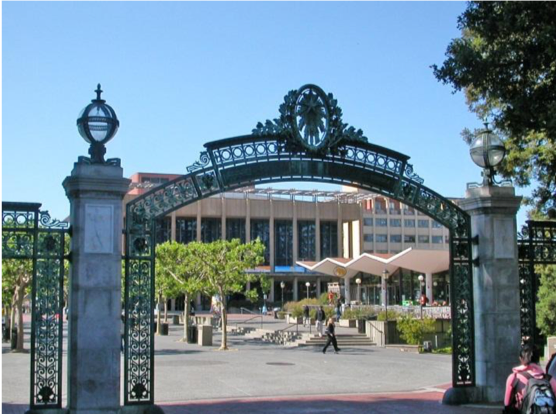
\includegraphics[width=\textwidth]{cal/sather_gate}
\end{minipage}
\hfill
\begin{minipage}{0.49\textwidth}
	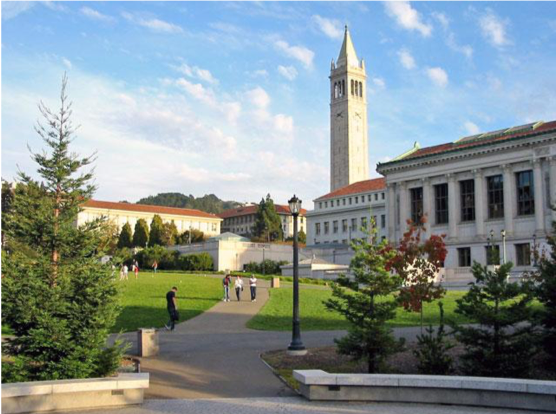
\includegraphics[width=\textwidth]{cal/campanile_glade}
\end{minipage}

\begin{minipage}{0.49\textwidth}
	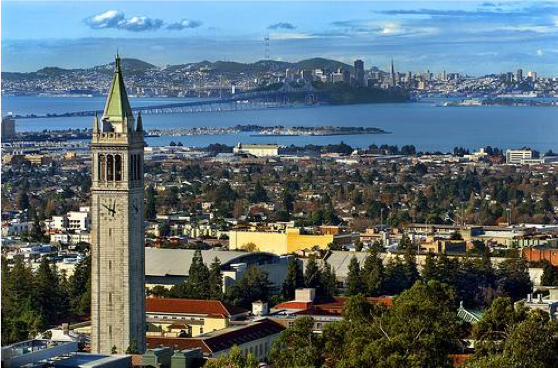
\includegraphics[width=\textwidth]{cal/campanile_hill}
\end{minipage}
\hfill
\begin{minipage}{0.49\textwidth}
	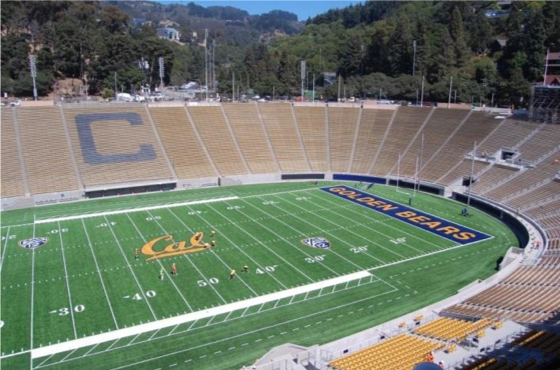
\includegraphics[width=\textwidth]{cal/memorial_stadium}
\end{minipage}
\vspace{0.5cm}
